\documentclass[a4paper,12pt]{article}
\usepackage[english]{babel}
\usepackage[utf8]{inputenc}

%
% For alternative styles, see the biblatex manual:
% http://mirrors.ctan.org/macros/latex/contrib/biblatex/doc/biblatex.pdf
%
% The 'verbose' family of styles produces full citations in footnotes, 
% with and a variety of options for ibidem abbreviations.
%
\usepackage{graphicx}
\usepackage{csquotes}
\usepackage[style=verbose-ibid,backend=bibtex]{biblatex}
\bibliography{sample}

\usepackage{lipsum} % for dummy text

\title{Reinforcement Learning for True Adaptive Traffic Signal Control}

\author{Shayan Amani}

\date{\today}

\begin{document}
\maketitle

\section{Introduction}
Interesting paper if you want to get a grasp on Q-learning in the context of an application-ready example. In this paper, authors tried to depict the possibilities that a reinforcement learning method (precisely Q-Learning) can introduce to control problems compared to conventional methods namely "prespecified models".

The authors pointed out the down sides of conventional model as follows:
\begin{itemize}
    \item Modeling environment before having any interaction with it (prespecified modeling).
    \item The high level of expertise needed to lay out such those models.
    \item Deteriorating generalization needed to cover all possible situations.
\end{itemize}

Later they have mentioned a set of advantages that a reinforcement learning approach such as:
\begin{itemize}
    \item Least dependency (even zero) on a predefined model.
    \item Ability of agent to improve itself by steadily learning from the surrounding environment.
\end{itemize}

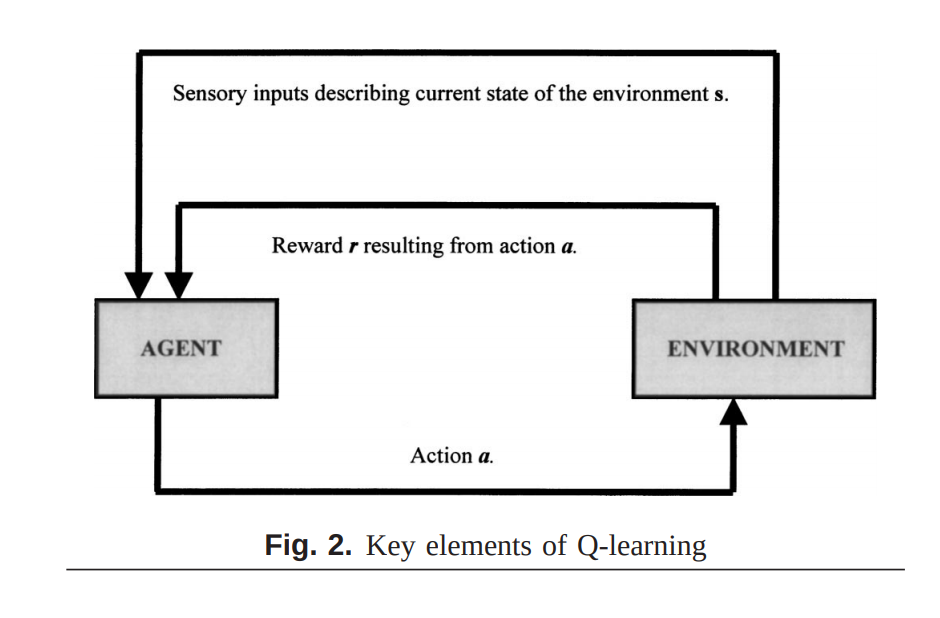
\includegraphics[width=1\columnwidth]{elements.png}


% This is an example citation \autocite{ginsberg}.
% \lipsum[1] % dummy text

% This is another example citation \autocite{brassard}.
% \lipsum[2] % dummy text

% This is a repeated citation \autocite{brassard}.
% \lipsum[3] % dummy text

% This is another example citation \autocite{adorf}.
% \lipsum[4] % dummy text 

\end{document}